\section{Multiple models}
We analyze the execution of multiple models on the \graicore{}.
In this scenario, we assume that each of these models fits on the \graicore{} individually and only a single model is present on the \graicore{} at a time.
Additionally, we assume an approach where the configuration and processing of the models occurs sequentially.
This approach avoids the complexities associated with parallelism and scheduling, making it easier to analyze performance.

To determine the required write bandwidth for configuring a model, we need the following parameters:
\begin{itemize}
    \item The input frame rate
    \item The amount of bytes to be written
    \item The frame processing latency
\end{itemize}

The amount of time we have available to configure the \graicore{} is dependent on the input frame rate and frame processing latency.
For example, for an input frame rate of \SI{60}{FPS}, we have a period of \SI{16.7}{ms} between every two frames.
Suppose we want to process every new incoming frame with a new model, all with a frame processing latency of \SI{5}{ms}. 
Due to the frame processing latency, we only have a time budget of \SI{11.7}{ms} to reconfigure the \graicore{} with the next model.

\Cref{fig:reconfig_time_line_ex} shows two example timelines of a good and a bad scenario when performing execution of multiple models in sequence.
$t_n$ indicates the time instance where the $n$th frame has been received by the \graicore{}, ready to be processed.
At $t_0$, the \graicore{} is already configured with an initial model.
In \cref{fig:correct_reconfig}, the \graicore{} uses a different model for each consecutive frame.
Each of these models have a similar processing latency and reconfiguration time.
After receiving and processing (P) the very first frame at $t_0$, it starts reconfiguration (C) to a new model.
Since the sum of the reconfiguration and processing time does not exceed the frame time ($t_{n+1} - t_{n})$, the frame processing latency (L) is equal for every incoming frame.
The invariant latency is desired and indicates a seamless reconfiguration.
\Cref{fig:incorrect_reconfig} has an increased reconfiguration time.
Now, the sum of the reconfiguration and processing time does exceed the frame time.
As a consequence, the frame processing latency increases for each incoming frame.
In the long run, this latency will grow to infinity.
Since the latency varies, this is an example of a non-seamless reconfiguration.

\begin{figure}[hbtp]
    \centering
    \subcaptionbox{Seamless reconfiguration \label{fig:correct_reconfig}}[\textwidth]{
        \begin{tikzpicture}[scale=0.5]
    \draw[] (6,0) -- (24,0);
    \draw[dashed, ->] (24,0) -- (25,0);
    \draw (6,0.5) -- (6,-0.5) node[below] {$t_{0}$};
    \draw (12,0.5) -- (12,-0.5) node[below] {$t_{1}$};
    \draw (18,0.5) -- (18,-0.5) node[below] {$t_{2}$};
    \draw (24,0.5) -- (24,-0.5) node[below] {$t_{3}$};

    \draw [pattern=north east lines, pattern color=gray, line width = 1pt, very thick] ($(6,0)$) rectangle ++($(1.5,1)$) node[midway] {P};
    \draw [pattern=north west lines, pattern color=gray, line width = 1pt, very thick] ($(7.5,0)$) rectangle ++($(3,1)$) node[midway] {C};
    \draw [decorate,decoration={brace,amplitude=6pt}]($(6,1.5)$) -- ++($(1.5,0)$) node [black,midway,above=6pt] {\tiny L};
    
    \draw [pattern=north east lines, pattern color=gray, line width = 1pt, very thick] ($(12,0)$) rectangle ++($(1.5,1)$) node[midway] {P};
    \draw [pattern=north west lines, pattern color=gray, line width = 1pt, very thick] ($(13.5,0)$) rectangle ++($(3,1)$) node[midway] {C};
    \draw [decorate,decoration={brace,amplitude=6pt}]($(12,1.5)$) -- ++($(1.5,0)$) node [black,midway,above=6pt] {\tiny L};
    
    \draw [pattern=north west lines, pattern color=gray, line width = 1pt, very thick] ($(18,0)$) rectangle ++($(1.5,1)$) node[midway] {P};
    \draw [pattern=north west lines, pattern color=gray, line width = 1pt, very thick] ($(19.5,0)$) rectangle ++($(3,1)$) node[midway] {C};
    \draw [decorate,decoration={brace,amplitude=6pt}]($(18,1.5)$) -- ++($(1.5,0)$) node [black,midway,above=6pt] {\tiny L};
\end{tikzpicture}

    }
    \subcaptionbox{Non-seamless reconfiguration \label{fig:incorrect_reconfig}}[\textwidth]{
        \begin{tikzpicture}[scale=0.5]
    \draw[] (6,0) -- (24,0);
    \draw[dashed, ->] (24,0) -- (25,0);
    \draw (6,0.5) -- (6,-0.5) node[below] {$t_{0}$};
    \draw (12,0.5) -- (12,-0.5) node[below] {$t_{1}$};
    \draw (18,0.5) -- (18,-0.5) node[below] {$t_{2}$};
    \draw (24,0.5) -- (24,-0.5) node[below] {$t_{3}$};

    \draw [pattern=north east lines, pattern color=gray, line width = 1pt, very thick] ($(6,0)$) rectangle ++($(1.5,1)$) node[midway] {P};
    \draw [pattern=north west lines, pattern color=gray, line width = 1pt, very thick] ($(7.5,0)$) rectangle ++($(5,1)$) node[midway] {C};
    \draw [decorate,decoration={brace,amplitude=6pt}]($(6,1.5)$) -- ++($(1.5,0)$) node [black,midway,above=6pt] {\tiny L};
    
    \draw [pattern=north east lines, pattern color=gray, line width = 1pt, very thick] ($(12.5,0)$) rectangle ++($(1.5,1)$) node[midway] {P};
    \draw [pattern=north west lines, pattern color=gray, line width = 1pt, very thick] ($(14,0)$) rectangle ++($(5,1)$) node[midway] {C};
    \draw [decorate,decoration={brace,amplitude=6pt}]($(12,1.5)$) -- ++($(2,0)$) node [black,midway,above=6pt] {\tiny L};
    
    \draw [pattern=north west lines, pattern color=gray, line width = 1pt, very thick] ($(19,0)$) rectangle ++($(1.5,1)$) node[midway] {P};
    % \draw [pattern=north west lines, pattern color=gray, line width = 1pt, very thick] ($(20.5,0)$) rectangle ++($(5,1)$) node[midway] {C};
    \draw [decorate,decoration={brace,amplitude=6pt}]($(18,1.5)$) -- ++($(2.5,0)$) node [black,midway,above=6pt] {\tiny L};
    \node[right] at (20.5,0.5) {\ldots};



\end{tikzpicture}
    }
    \caption{
        Example time lines of reconfiguration with multiple models.
    }
    \label{fig:reconfig_time_line_ex}
\end{figure}

We calculate the required effective bandwidth for configuring model $m$ with \cref{eq:multiple_models_bandwidth}.
\begin{equation}
    \bandwidth_m = \frac{d_m}{f^{-1} - l_m}
    \label{eq:multiple_models_bandwidth}
\end{equation}

\begin{eqexpl}[15mm]
    \item{$\bandwidth_m$} required effective bandwidth for writing model $m$
    \item{$d_m$} amount of bytes to write for model $m$
    \item{$f$} input frame rate
    \item{$l_m$} frame processing latency for model $m$
\end{eqexpl}

In the worst-case scenario, we have to configure the \graicore{} with a model requiring to write the total capacity of the \graicore{} (\SI{36}{\mebi\byte}).
In this particular instance, we require a minimum write bandwidth of $\SI{3086}{\mebi\byte\per\second}$\footnote{$\frac{\SI{36}{\mebi\byte}}{\frac{1}{\SI{60}{\hertz}} - \SI{5}{\milli\second}} \approx \SI{3086}{\mebi\byte\per\second}$} for $\SI{60}{FPS}$, assuming the model's processing time is \SI{5}{ms}.
% Note that this bandwidth number does not include any overhead induced by communication protocols. Therefore, in practice, the required minimum bandwidth is higher. 
This bandwidth calculation provides a baseline for the effective bandwidth.
In practice, the actual bandwidth needed will be higher due to overhead introduced by various factors, including the specific communication protocol(s) used.
For example, using the network packet format of the current \confignoc{}, 50\% of the total data transferred is overhead.
The system then requires an actual bandwidth of double the effective bandwidth.

Using the previous example, \cref{fig:frame_rate_versus_time_budget} shows that an increase in frame rate decreases the available time budget for reconfiguration.
\Cref{tab:common_fps} shows a list of common video frame rates with their associated reconfiguration time budget.
A frame rate with zero or negative time budget means that the \graicore{} cannot be reconfigured seamlessly for a video with the corresponding frame rate.
Exceeding this time budget results into a delayed output which is undesirable since it negatively affects the user experience.
At a frame rate of $\SI{200}{FPS}$, the time budget is exactly zero, indicating that this represents the tight upper bound.

\begin{figure}[htbp]
    \centering
    \begin{subfigure}[b]{0.48\textwidth}
        \begin{adjustbox}{width=\linewidth}
        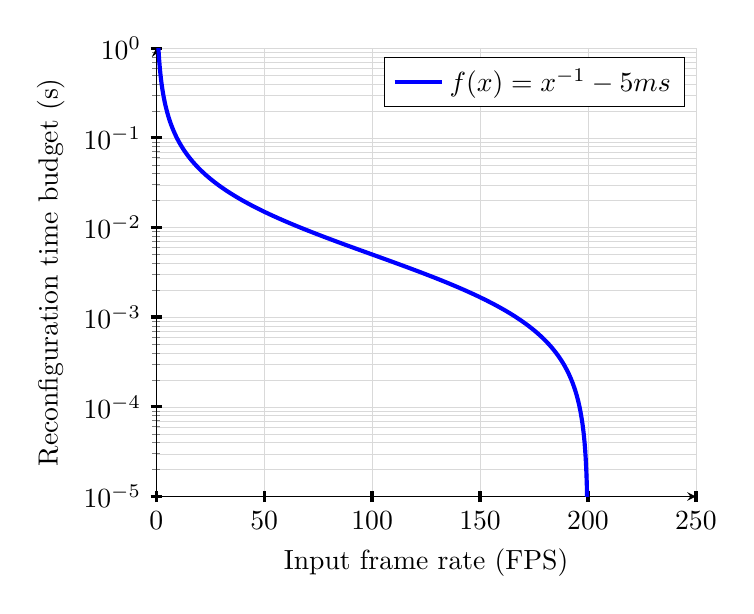
\begin{tikzpicture}
\begin{semilogyaxis}[
    xmin=0, xmax=250,
    ymin=0.00001, ymax=1,
    axis lines = left,
    xlabel = {Input frame rate (FPS)},
    ylabel = {Reconfiguration time budget (s)},
    ymajorgrids=true,
    grid=both,
    % grid style=dashed,
    grid style={line width=.1pt, draw=gray!30},
    every major tick/.append style={very thick, major tick length=4pt, black},
]

% 16 bits
\addplot[
    domain=0:250, 
    samples=1000, 
    color=blue,
    line width=1.5pt
]
{1/x - 0.005};
% \addlegendentry{$B(f) = f^{-1} - \SI{5}{ms}$}
\addlegendentry{$f(x) = x^{-1}  - \SI{5}{ms}$}
\end{semilogyaxis}
\end{tikzpicture}

        \end{adjustbox}
        \caption{An increase in frame rate lowers the reconfiguration time budget}
        \label{}
    \end{subfigure}
    \hfill
    \begin{subfigure}[b]{0.48\textwidth}
        \begin{tabular}{@{}ll@{}}
        \toprule
        Frame rate (FPS) & Reconf. budget (ms) \\ \midrule
        15               & 61.7                \\
        24               & 36.7                \\
        30               & 28.3                \\
        60               & 11.7                \\
        120              & 3.3                 \\
        200              & 0.0                 \\
        240              & -0.8                \\ \bottomrule
        \end{tabular}
        \caption{Reconfiguration time budget for different common video frame rates}
        \label{tab:common_fps}
    \end{subfigure}
    \caption[]{Input frame rate versus reconfiguration time budget}
    \label{fig:frame_rate_versus_time_budget}
\end{figure}

If we have a set of different models (with varying sizes and processing times) we want to switch between, the system needs to be able to reach the highest required writing bandwidth:
\begin{equation}
    \bandwidth = \max\{\,m \in M \mid \bandwidth_m \,\} 
\end{equation}

